%Demonstra como foi realizado o trabalho
%• Pesquisas bibliográficas: sempre com as referências
%• Modelagem
%• Sistema gerado
%• Testes de desempenho/avaliação
\chapter{Métodos}
\noindent
\section{Bag of Words}
%https://www3.nd.edu/~dchiang/teaching/nlp/2015/notes/chapter1v2.pdf
%https://towardsdatascience.com/machine-learning-nlp-text-classification-using-scikit-learn-python-and-nltk-c52b92a7c73a
Bag of words não se trata de modelo de classificação por completo, mas sim de uma estratégia de representação do texto em que a sequência de palavras é desconsiderada. Dessa maneira, o texto é simplificado para uma lista de palavras distintas e a respectiva contagem de ocorrência de cada uma delas. A principal vantagem dessa estratégia é a sua simplicidade de representação computacional, sendo atrativa para a aplicação direta de algoritmos de aprendizado de máquinas.

Contudo, para se obter uma melhor eficiência dessa estratégia, pode ser necessário aplicar outras técnicas que mitiguem a perda de informação causada pelo bag of words. Uma dessas técnicas é a remoção de palavras vazias (stop words), pois essas palavras são utilizadas apenas para a conexão de ideias em uma frase como preposições, artigos e conjuções e não contribuem como fonte de informação no texto. Além disso, as palavras vazias ocorrem com alta frequência e possuem destaque ilusório na representação colapsada do bag of words. Outra técnica que também pode ser empregada é a stemização (stemming) que corresponde a remoção dos sufixos das palavras, pois estes fazem com que palavras que deveriam ser sinônimas na representação bag of words sejam contabilizadas separadamente. Ao remover os sufixos como gênero, tempo e número, palavras que acrescentam a mesma informação ao texto terão suas respectivas contagens somadas em uma única palavra sem os sufixos.

\section{Redes Neurais Artificiais}
Redes Neurais Artificiais são mecanismos de aprendizado de máquina inspirados nos sistemas neurais biológicos. Seu funcionamento se dá atravez de neurônios artificiais.

\subsection{Neurônios}

\begin{figure}[!ht]
	\centering
	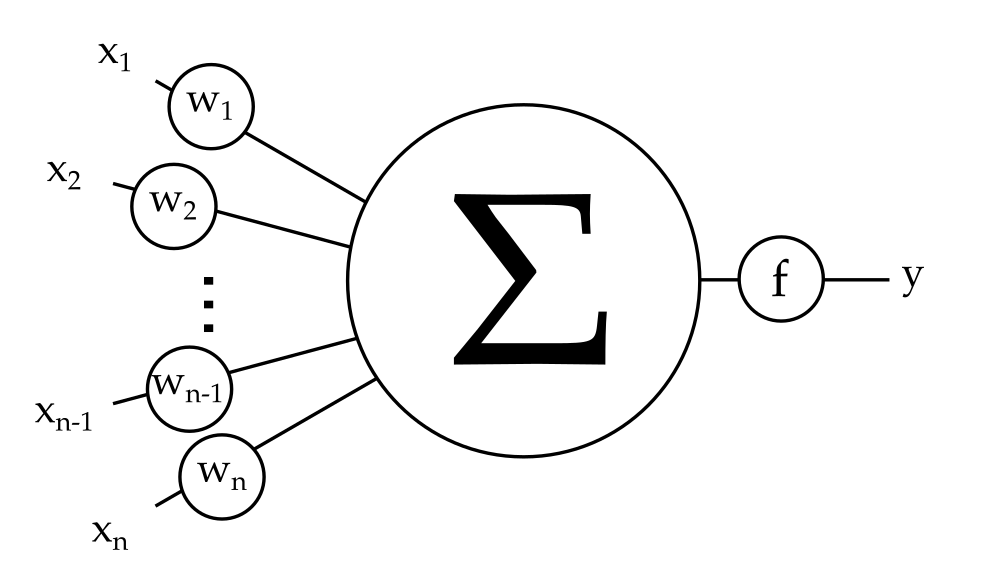
\includegraphics[width=0.6\textwidth]{figures/neuron.png}   
	\caption{Neurônio artificial}
	\label{fig:neuron}
\end{figure}


Conforme a figura \ref{fig:neuron}, um neurônio artificial é uma função $y:\mathbb R^n \rightarrow \mathbb R$ com entrada $\vec x = <x_1,x_2,x_3,\dots,x_n>$ e saída $y = f(\sum\limits_{i=1}^n x_iw_i)$.

\subsection{Camadas}
Camadas de uma rede neural são concatenações de neurônios que formam uma função com múltiplas entradas e saídas.

\subsection{Redes neurais}
Redes neurais são listas ordenadas de camadas formando uma função conjugada. Existem variações de redes neurais não contempladas pelas definições acima, mas todas serão tratadas separadamente.

%https://www.coursera.org/specializations/deep-learning
%https://www.coursera.org/learn/machine-learning
\subsection{Word Embedings}

Word embedding é a representação de palavras de um vocabulário em um espaço n-dimensional de números reais. Isso permite que palavras que são usadas de maneira similar tenham representações similares, de maneira a capturar o significado de cada palavra de acordo com a sua posição no espaço n-dimensional. Cada palavra é mapeada a um vetor e os valores desse vetor são obtidos a partir de um treinamentos que, em geral, envolvem redes neurais como o skip-gram utilizado na implementação word2vec, \cite{DBLP:journals/corr/MikolovSCCD13}.

\subsection{Redes Neurais Convolucionais}
Redes convolucionais são variações de redes neurais inspiradas no córtex visual. São baseadas em convoluções.

\begin{figure}[!ht]
	\centering
	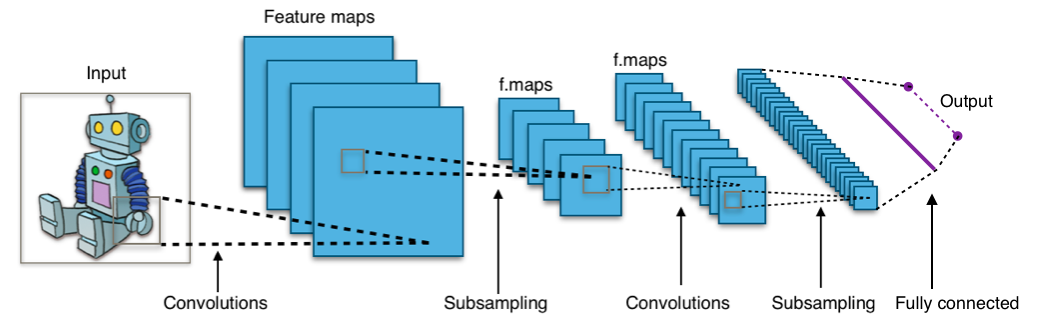
\includegraphics[width=0.6\textwidth]{figures/cnn.png}   
	\caption{Rede Neural Convolucional}
	\label{fig:cnn}
\end{figure}

\subsection{Convoluções}
Sejam os vetor $\vec u = <u_1,u_2,\dots, u_n >$ e $\vec v = <v_1,v_2,\dots, v_m>$ com $\vec u \in \mathbb R^n$ e $\vec v \in \mathbb R^m$. Entende-se como convolução de $\vec v$ em $\vec u$ o vetor $\vec c = <\dots \sum\limits_{TODO}^{TODO} u_iv_j \dots>$.



%http://cs231n.github.io/
%http://cs224d.stanford.edu/syllabus.html
%https://www.coursera.org/learn/convolutional-neural-networks
\subsection{Redes Neurais Recorrentes}
%http://cs224d.stanford.edu/syllabus.html